%%% Décommenter pour une présentation
\documentclass{beamer}
%%%

%%% Décommenter pour avoir un article
%\documentclass[handout]{beamer}
%\usepackage{pgfpages}
%\pgfpagesuselayout{2 on 1}[a4paper,border shrink=5mm]
%\setbeameroption{show notes on second screen=bottom} % Beamer manual, section 19.3
%%%

%%%%%%%%%%%%%%%%%%%%%%%%%%%%%%%%%%%%%%%%%%%%%%%%%%%%%%%%%%%%%%%%%%%%%%
% NE PAS MODIFIER CETTE PARTIE

\usetheme{Warsaw}
\usepackage[utf8]{inputenc}
\usepackage[T1]{fontenc}
\usepackage{amsmath}
\usepackage{amsfonts}
\usepackage{amssymb}
\usepackage{graphicx}
\usepackage{listings}
\usepackage{hyperref}

\graphicspath{{graphics/}}

\hypersetup{pdfstartview={Fit}}



\AtBeginSection[]{
  \begin{frame}
  \vfill
  \centering
  \begin{beamercolorbox}[sep=8pt,center,shadow=true,rounded=true]{title}
    \usebeamerfont{title}\insertsectionhead\par%
  \end{beamercolorbox}
  \vfill
  \end{frame}
}

\setbeamertemplate{note page}[plain] % Beamer manual, section 19.1
\newlength{\parskipbackup}
\setlength{\parskipbackup}{\parskip}
\newlength{\parindentbackup}
\setlength{\parindentbackup}{\parindent}
\newcommand{\baselinestretchbackup}{\baselinestretch}
\usetemplatenote{\rmfamily \scriptsize%
  \setlength{\parindent}{1em} \setlength{\parskip}{1ex}%
  \renewcommand{\baselinestretch}{1}%
  \noindent \insertnote%

  \setlength{\parskip}{\parskipbackup}%
  \setlength{\parindent}{\parindentbackup}%
  \renewcommand{\baselinestretch}{\baselinestretchbackup}%
}

\logo{
	
\includegraphics[scale=0.1]{SPCL.png}
} 
\institute[ETH Zürich]{\textbf{ETH Zürich}}




%%%%%%%%%%%%%%%%%%%%%%%%%%%%%%%%%%%%%%%%%%%%%%%%%%%%%%%%%%%%%%%%%%%%


%TODO : PARTIE A MODIFIER 

\date{October 2018}	

\author{
    Th. Cambier
    R. Dang-Nhu
    Th. Dardinier
    C. Trassoudaine
}
\title{
	\textbf{Minimum Spawning Tree}\\
	-\\ 
	\textit{DPHPC}
}




\begin{document}

\frame{\titlepage}
\frame{\tableofcontents}

%%%%%%%%%%%%%%%%%%%%%%%%%%%%%%%%%%%%%%%%%%%%%%%%%%%%%%%%%%%%%%%%%%%%
% SECTION 1
%%%%%%%%%%%%%%%%%%%%%%%%%%%%%%%%%%%%%%%%%%%%%%%%%%%%%%%%%%%%%%%%%%%%

\section{Problem definition}
\begin{frame}
\frametitle{The MST problem}
\end{frame}

\subsection{Concepts}
\begin{frame}
\frametitle{Concepts}
\end{frame}

\subsection{Use cases}

\begin{frame}
(Somewhat) realistic use-cases and input sets?

\begin{itemize}
\item[•] $G(n, p)$
\item[•] Preferential attachment
	\begin{itemize}
	\item Social networks
	\end{itemize}
\end{itemize}
\end{frame}

%%%%%%%%%%%%%%%%%%%%%%%%%%%%%%%%%%%%%%%%%%%%%%%%%%%%%%%%%%%%%%%%%%%%
% SECTION 2
%%%%%%%%%%%%%%%%%%%%%%%%%%%%%%%%%%%%%%%%%%%%%%%%%%%%%%%%%%%%%%%%%%%%

\section{Algorithms}
\subsection{Prim}
\begin{frame}
\frametitle{Prim}
\end{frame}
\subsection{Kruskal}
\begin{frame}
\frametitle{Kruskal}
\end{frame}
\subsection{Borůvka (Sollin)}
\begin{frame}
\frametitle{Borůvka (Sollin)}
\end{frame}
\subsection{Others}
\begin{frame}
\frametitle{A few ideas}
\end{frame}
\begin{frame}
\frametitle{Correctness}
How to verify correctness of the parallelization?
\end{frame}

%%%%%%%%%%%%%%%%%%%%%%%%%%%%%%%%%%%%%%%%%%%%%%%%%%%%%%%%%%%%%%%%%%%%
% SECTION 3
%%%%%%%%%%%%%%%%%%%%%%%%%%%%%%%%%%%%%%%%%%%%%%%%%%%%%%%%%%%%%%%%%%%%

\section{Environment}
\begin{frame}
\frametitle{Architecture}
\begin{figure}
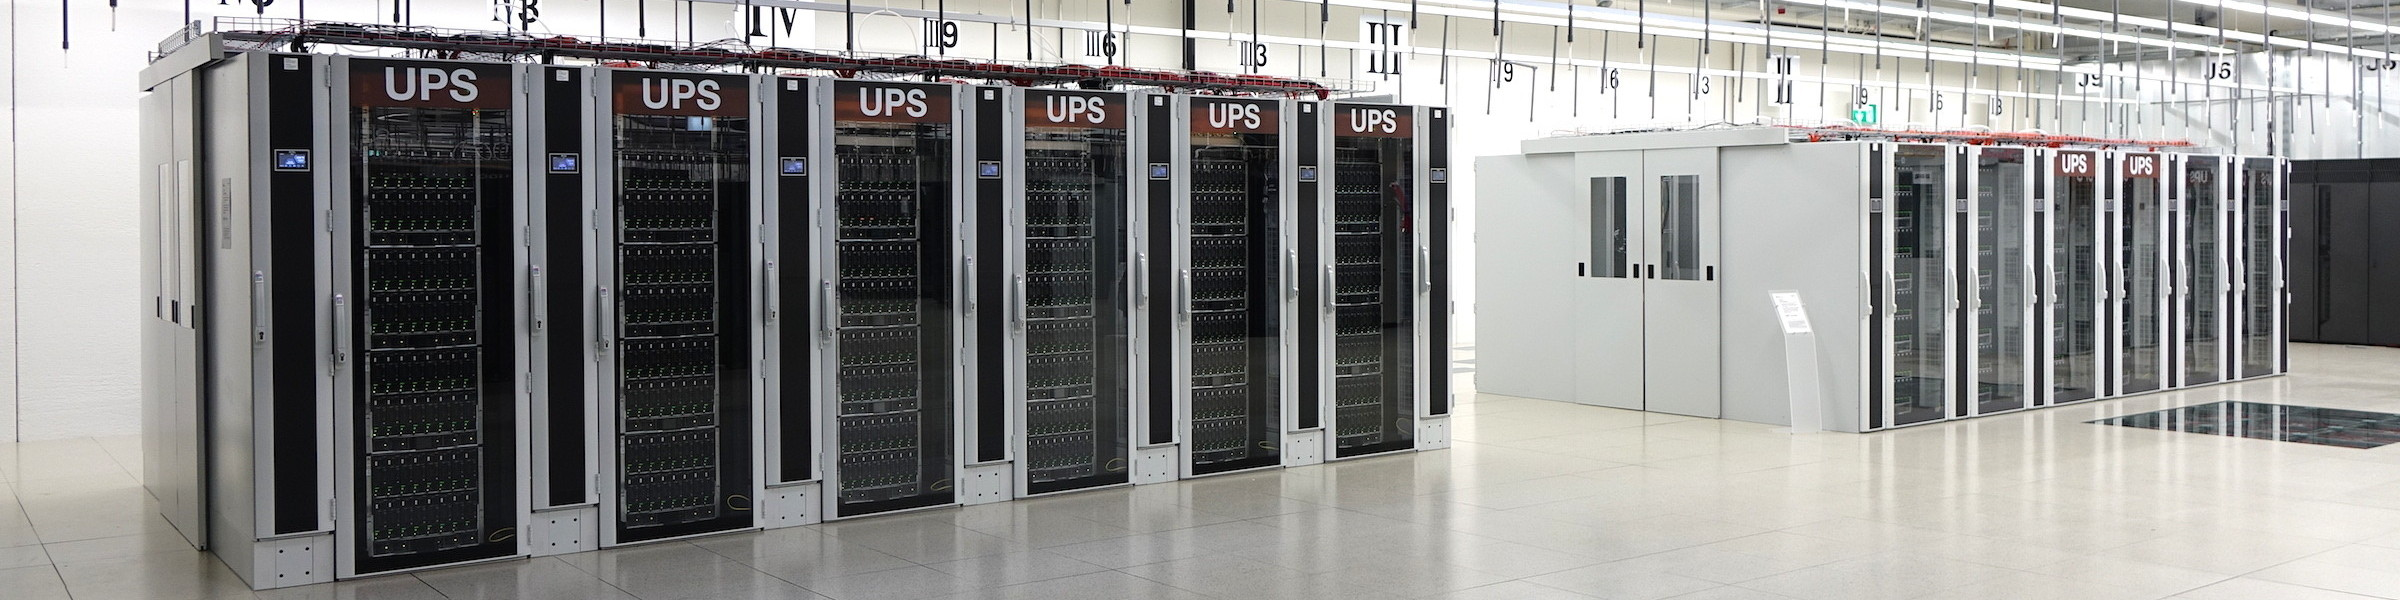
\includegraphics[scale=0.4]{EULER.jpg}
\end{figure}

\centering{ \large EULER Cluster }

\vspace{.5 cm}

Xeon E$x, x\in\{3, 5, 7\}$ ; x86\_64 architecture
\vfill
{
\tiny
Source : 
\url{https://scicomp.ethz.ch/wiki/Euler}
}
\end{frame}
\begin{frame}
\frametitle{Tools}
\begin{columns}
\begin{column}{.4\linewidth}

\includegraphics[scale=.1]{OPENMP.png}
\end{column}

\begin{column}{.6\linewidth}
\begin{itemize}
\item[•] C++ (gcc, mpicc wrapper)
\item[•] OMP (shared memory)
\end{itemize}
\end{column}
\end{columns}

\end{frame}

%%%%%%%%%%%%%%%%%%%%%%%%%%%%%%%%%%%%%%%%%%%%%%%%%%%%%%%%%%%%%%%%%%%%
% SECTION 4
%%%%%%%%%%%%%%%%%%%%%%%%%%%%%%%%%%%%%%%%%%%%%%%%%%%%%%%%%%%%%%%%%%%%

\section{Benchmarking}
\subsection{Reference, baseline, tools}
\begin{frame}

\textbf{\Large Tools} 

\begin{itemize}
\item[•] \textbf{Measures :} LibSciBench library
\item[•] \textbf{Interpretation :} LibSciBench's R scripts
\end{itemize}

{
\tiny
Ref : 
\url{https://spcl.inf.ethz.ch/Research/Performance/LibLSB/}
}

\vfill

\textbf{\Large Baseline}

\begin{columns}
\begin{column}{0.3\linewidth}
\begin{center}
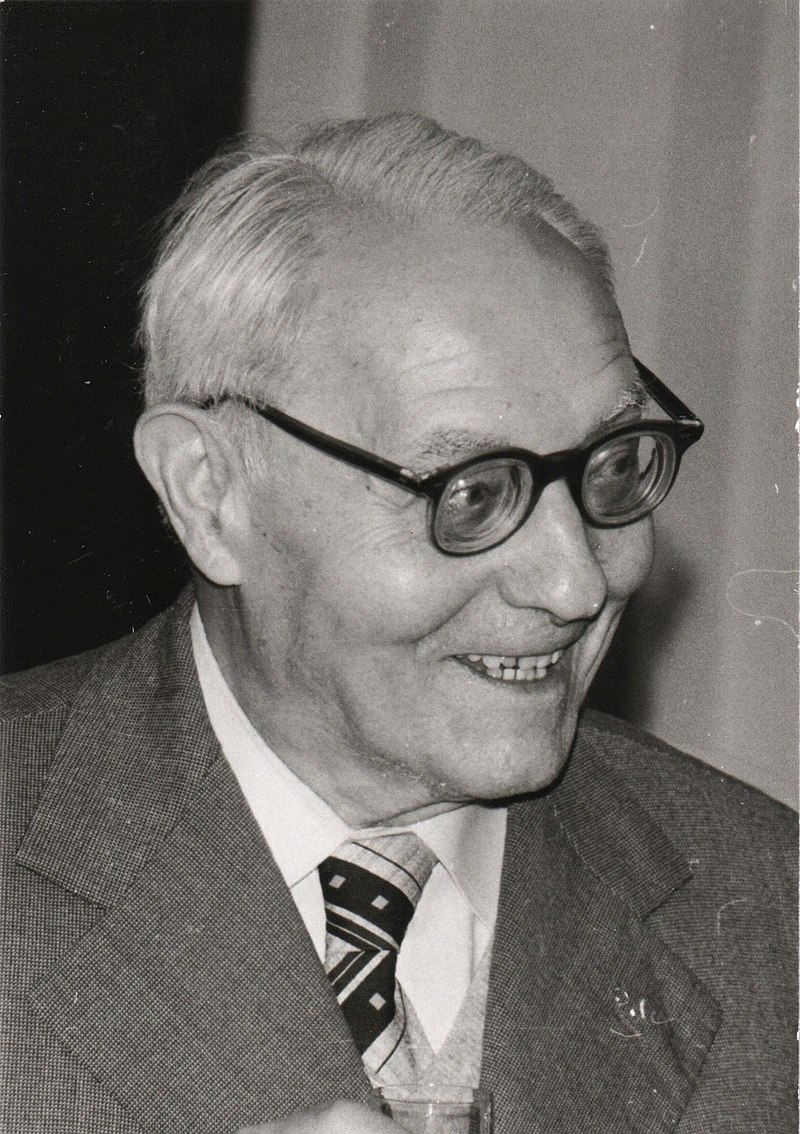
\includegraphics[scale=.05]{Boruvka.jpg}
\end{center}
\end{column}
\begin{column}{0.7\linewidth}
\begin{center}
Borůvka's serial algorithm

$O(E \cdot log(V))$
\end{center}
\end{column}
\end{columns}
{\tiny \url{https://en.wikipedia.org/wiki/Otakar_Bor\%C5\%AFvka}}

\end{frame}


\end{document}